\subsection[]{Nebel- und Blasenkammer}

%___________________________________________________________________________________________________

\begin{frame}{Nebelkammer}
	Erfindung 1911 durch Charles Wilson
	\vspace{0.7cm}
	\begin{block}{Kammer mit übersättigtem Wasserdampf}
		\begin{itemize}
		  \item Ionisierende Strahlung bildet Ionen-Elektronen-Paare im Gas
		  \item Ionen wirken als Kondensationskeim
		  \item Kondensierte Tröpfchen bilden sichtbaren Kondensstreifen 
		  \item Fotografie der Kondensstreifen für spätere Spurrekonstruktion
		\end{itemize}
	\end{block}
	\vspace{0.7cm}
	Später: Übersättigte Luft-Alkohol-Gemische\\

\end{frame}

%___________________________________________________________________________________________________



\begin{frame}{Funkenkammer - Aufbau}
    \begin{columns}[T]
    
	    \column{.5\textwidth}
			\begin{figure}[htbp]
			  \centering
			  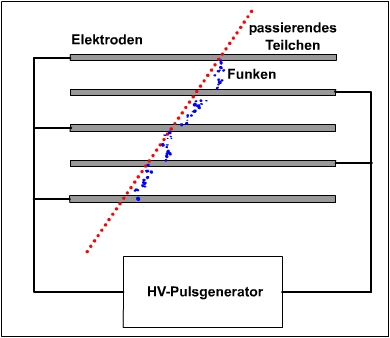
\includegraphics[width=\textwidth]{prinzipfk.jpg}
			  \caption{Aufbau einer Funkenkammer [gfa]}
			\end{figure}
			
	    \column{.5\textwidth}
	    	\begin{itemize}
			  \item Zwischen mehreren leitenden Platten in Edelgas liegt abwechselnde HV an
			  \item Ionisierende Strahlung bildet Ionen-Elektronen-Paare im Gas
			  \item Funken springen zwischen Platten über - entlang der Ionisationsspur
			  \item HV meist getriggert durch Szintillatoren
			\end{itemize}
    \end{columns}
\end{frame}

%___________________________________________________________________________________________________

\begin{frame}{Nebel- und Funkenkammer}
    \begin{columns}[T]
	    \column{.5\textwidth}
	    \center{Nebelkammer [gnk]}
			\begin{figure}[htbp]
			  \centering
			  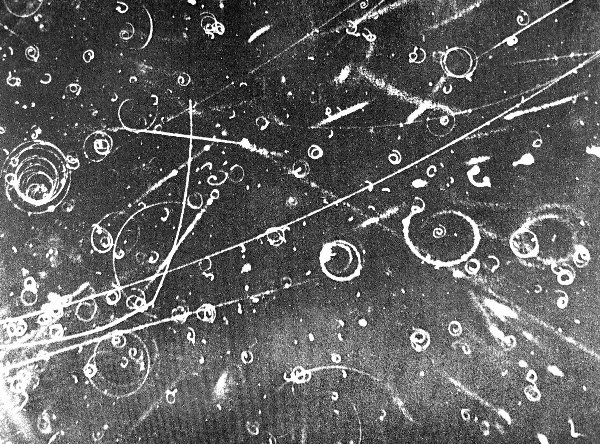
\includegraphics[width=\columnwidth]{nebelkammer.jpg}
			\end{figure}
			
	    \column{.5\textwidth}
	    \center{Funkenkammer [gfk]}
	    	\begin{figure}[htbp]
			  \centering
			  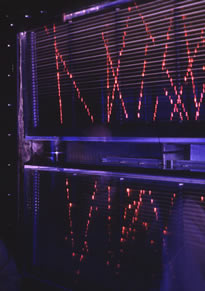
\includegraphics[width=\columnwidth*2/3]{funkenkammer.jpg}
			\end{figure}
    \end{columns}
\end{frame}

\begin{frame}{Nebel- und Funkenkammer}
	    \center{Entdeckung des Positrons (1932) [epo]}
			\begin{figure}[htbp]
			  \centering
			  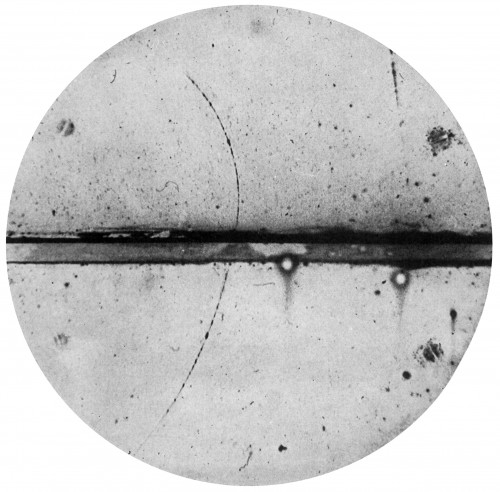
\includegraphics[scale=0.3]{positron.jpg}
			\end{figure}
		Weiterhin: Nachweis Comptoneffekt, Paarerzeugung/-vernichtung, \ldots
\end{frame}

% \begin{frame}{Blasenkammer}
% 	Erfindung 1952 durch Donals A. Glaser
% 	\begin{block}{Ähnliches Prinzip wie Nebelkammer}
% 		\begin{itemize}
% 		  \item Metastabiler Zustand von flüssigem Wasserstoff bei adiabatischer
% 		  Druckänderung
% 		  \item Ionen wirken als Siedekeim
% 		  \item Entstandene Bläschen visualisieren Teilchenspur 
% 		  \item Fotografie der Blasenspuren für spätere Rekonstruktion
% 		\end{itemize}
% 	\end{block}
% \end{frame}
% 
% %___________________________________________________________________________________________________
% 
% \begin{frame}{Blasenkammer - Aufbau}
%     \begin{columns}[T]
%     
% 	    \column{.6\textwidth}
% 			\begin{figure}[htbp]
% 			  \centering
% 			  \includesvg[svgpath=bilder/, width=\textwidth]{Blasenkammer}
% 			  \caption{Blasenkammer mit B-Feld [wbk]}
% 			\end{figure}
% 			
% 	    \column{.45\textwidth}
% 	    	\begin{enumerate}
% 			  \item Kurz vor Messung wird Druck verringert
% 			  \item Temperatur nun oberhalb des Siedepunktes
% 			  \item Kameras bilden Blasenspuren ab
% 			  \item 3D-Rekonstruktion der Spuren möglich
% 			  \item Druck wird wieder erhöht damit sich Blasen wieder lösen  
% 			\end{enumerate}
%     \end{columns}
% \end{frame}

%___________________________________________________________________________________________________

\begin{frame}{Nebel- und Funkenkammern}
    \begin{columns}[T]
		\column{.45\textwidth}
			\textbf{Vorteile}		
			\vspace{0.7cm}
			\begin{itemize}
			  \item Bahnen direkt sichtbar (einfache Rekonstruktion)
			  \item Günstig
			  \item Voller Raumwinkel bei Nebelkammer
			\end{itemize}	
	    \column{.5\textwidth}
	    	\textbf{Nachteile}
	    	\vspace{0.7cm}
	    	\begin{itemize}
			  \item Langsame Bildung der Spur (Nebelkammer)
			  \item Nur Nebelkammer kann kontinuierlich betrieben werden
			  \item Viel Materie (WW mit Teilchen)
			  \item Ortsauflösung Funkenkammer: $O(1 mm)$
			\end{itemize}
    \end{columns}
    \vspace{1cm}
    Heute: Nur noch für demonstrative Zwecke
\end{frame}